\chapter{Fundamental Concepts}
%aj instead of theory I would suggest to name it background 
This chapter presents fundamental concepts that help understand the methodologies used during the course of this project. In section \ref{sec:T:RoboticConcepts}, the reader will be presented with robotic concepts that regards both mobile robotics and robotic manipulators. Then, in section \ref{sec:T:AutonomousNavigation}, theory around autonomous mobile robots are presented. Finally, in section \ref{sec:T:MachineVision}, some theory about computer vision systems for object detection and pose estimation will be explained. 
% related to unmanned ground vehicle (UGV) for the application of warehouse automation. write in the verybeginning about the building block for this application - perception, autonomous navigation with collission detection and  avoidance, object detection and localization, robotic manipulation for pick and place. Then each of these becomes a section

% aj - presents. Not is future but in simple present tense. something like this
% This chapter presents the ovelying thoery behind the autonomous warehous functionalities namely ... a,b,c .. in chapter 1. Starting with the fundamental conpept of use of unmanned ground vehicle (UGV) for warehouse automation, then we describe the autonomous navigation ......Finally we intergrate individual functionalities to achieve warehouse automation.

\section{Robotic Concepts} \label{sec:T:RoboticConcepts}
This thesis is focused on a mobile robotic platform with a mounted robotic manipulator. Both mobile robotics and manipulator robotics share some fundamental concepts that forms the basis of robotics. This section will touch onto some of these concepts to give the reader a level of understanding of robotics needed to better understand the methodologies in the thesis. 
%More in depth description of these concepts and may more, can be found in \cite{LynchKevin2017Mr:m}.

A robot consists of rigid bodies, called links, connected through joints. The links can be arranged in whichever configurations that suits the needs of the designer. For example, a serial configuration could form the familiar manipulator arm, or a parallel configuration could form a mobile robot like the differential drive robot discussed in section \ref{sec:T:AN:MRD:DifferentialDriveRobots}. Robotic joints are often, but not limited to, revolute joints. These joints are commonly driven by actuators such as electric motors.

\subsection{Degrees of Freedom}
Robotics often refers to Degrees Of Freedom (DOF). DOF refers to the smallest number of real-valued coordinates needed to define the configuration of a robot \cite{LynchKevin2017Mr:m}. When comparing a mobile robot to a manipulator, the position of the mobile robot's chassis on a plane can be determined by three real-valued coordinates, ($x,y,\theta$). The mobile robot is therefore called a 3-DOF robot. Whereas a robotic manipulator, dependent on the amount and types of joints, could need a much larger amount of coordinates to determine it's configuration. The DOF of a mechanical system, and thus, a robot, can be determined by the use of Gr\"{u}bler's formula.  Gr\"{u}bler's formula states that for $N$ links, where the ground is also regarded a link, $J$ is the number of joints, $m$ is the number of DOF-s for a rigid body(3 for 2D, 6 for 3D), $c_i$ is the number of constrains  provided by joint $i$ and $f_i$ is the number of freedoms provided by joint $i$. The number of DOFs for a mechanical system then becomes

\begin{align}
\label{ec:DOFs}
    dof = m(N-1) -  \sum_{i=1}^{J} c_i \\
    = m(N-1) - \sum_{i=1}^{J}(m-f_i) \\
    = m(N-1-J) + \sum_{i=1}^{J}f_i.
\end{align}

Note that Gr\"ubler's formula may not give an accurate result in cases where the joint constraints are not independent\cite{LynchKevin2017Mr:m}.

\subsection{Configuration Space}
The configuration of a mechanical system is a specification of all it's points \cite{LynchKevin2017Mr:m}. All configurations a robot can reach is called it's configuration space, $C_{space}$. The dimension of $C_{space}$ is determined by the robot's DOF. Not all configurations in the $C_{space}$ are free of obstacles. Therefore, the $C_{space}$ can be divided into free space, $C_{free}$ and $C_{obs}$. For a mobile robot moving in a planar environment, $C_{space}$ can be represented as a 2D map, where $C_{obs}$ are obstacles (walls, furniture etc.) and $C_{free}$ is clear area where the mobile robot can move. For robotic manipulators, $C_{space}$ definitions quickly becomes more complicated. A simple example is shown in figure \ref{fig:T:RC:CSpace}, where a two-link planar arm is illustrated in physical space \textbf{a)} and $C_{space}$ \textbf{b)}. The robot should move from start to finish, it's path is illustrated in $C_{space}$. It can be seen from this figure that the robot's configuration can be determined by two coordinates, ($\theta_1, \theta_2$). Using Gr\"ubler's formula, the robot's DOF becomes $dof=3(3-1-2)+2=2$. Which corresponds with the fact that the dimension of $C_{space}$ is determined by the robot's DOF.

\begin{figure}[htp]
  \centering
  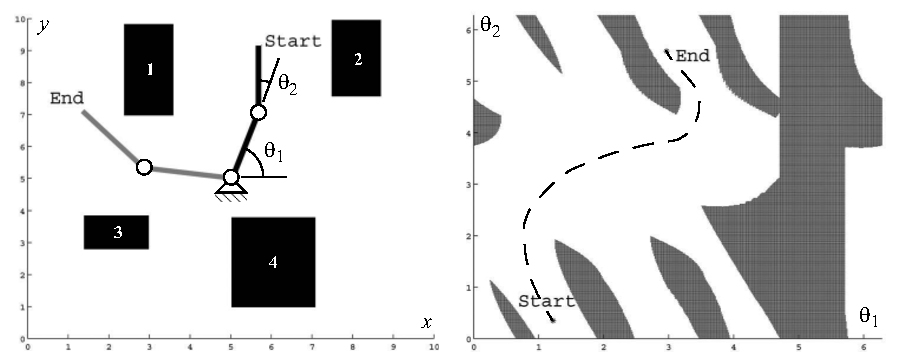
\includegraphics[width = 0.8\textwidth]{Figures/figConfSpace.pdf}
  \caption{Two link planar robot in physical space, \textbf{a)} and configuration space \textbf{b)}. The robot should move from start to finish, it's path is represented in \textbf{b)}. The configuration of the robot can be determined in configuration space by ($\theta_1, \theta_2$). Figure from \cite{SiegwartRoland2011Itam}.}
  \label{fig:T:RC:CSpace}
\end{figure}

\subsection{Kinematics}
Kinematics is the most basic study of how mechanical systems behave\cite{SiegwartRoland2011Itam}. In kinematics, the motion of a mechanical system is studied from a purely geometric point of view, meaning that forces and masses are neglected. In robotics, kinematics is fundamental for robotic control. For a robotic system to move through the environment, it need knowledge about how its links are put together and how they move relative to each other. Kinematics is largely divided into forward and inverse kinematics. 

Forward kinematics studies the way a mechanical system reacts to position, velocity or acceleration inputs in it's joints. For a robotic manipulator, the pose of the end-effector is solely determined by the joint positions. 

Inverse kinematics studies what the position of a mechanical system's joints would need to be in order to achieve a given pose in one of it's rigid bodies. Inverse kinematics is complicated and there are often more than one solution as robots might often be able to reach a defined pose in different configurations.

\subsection{Path Planning} \label{sec:T:RC:PathPlanning}
Path planning involves finding a trajectory that the robot can follow to reach it's goal \cite{SiegwartRoland2011Itam}. This applies to both robotic manipulators and mobile robots. Path planning in mobile robotics draws from the extensive research done in this area for robotic manipulators \cite{SiegwartRoland2011Itam}. However, path planning for mobile robots is usually far less complex than that of manipulators due to the reduced degrees of freedom \cite{SiegwartRoland2011Itam}. There are numerous different path planning algorithms available, two of the more popular path planning algorithms for use in mobile robotics is Djikstra's Algorithm \cite{DijkstraE.W1959Anot}, which computes the optimal path between a point and all other points in the configuration space, and A Star (A*) \cite{HartNilsson1968}. A* is often much faster at finding a path, however, it might not necessarily find the optimal path.

Popular path planners for manipulators include Rapidly Exploring Random Tree Star (RRT*) \cite{KaramanSertac2011Safo}, an optimal solution to Rapidly Exploring Random Tree(RRT) \cite{LaValleStevenM.2001RKP}, and Probabilistic Road Maps (PRM) \cite{KavrakiL.E.1996Prfp}, which also has an optimal variation, (PRM*)\cite{KavrakiL.E.1996Prfp}. These planners are effective at handling high complexity $C$ spaces relatively rapidly\cite{LynchKevin2017Mr:m}. As a side note, robotic manipulators are optimised for speed in order to reduce costs in a production line. This requires the dynamics of the system to be taken into account when planning the motion of the manipulator, significantly increasing the complexity of the problem. Path planning including the dynamics of the system is often referred to as motion planning \cite{LynchKevin2017Mr:m}.

\subsection{Robotic Software Platforms} \label{sec:RS:RoboticSooftwarePlatforms}
Robotic software platforms, often called middleware, are software solutions that aims at decomposing complex software into simpler and more manageable parts. The go-to solution for such a system in research over the last years is Robot Operating System (ROS) \cite{QuigleyROS}. The name suggests that this is a computer operating system (OS), but \cite{QuigleyROS} characterise this as a communication layer on top of the OS. ROS is built upon nodes, messages, topics and services, illustrated in figure \ref{fig:T:RC:Nodes}. Nodes are processes that perform the computation. Nodes communicate by structuring their data into messages, which is a strictly defined data structure. For a node to send a message, it has to publish this message to a topic. A topic is just a string, for example "scan" or "points". Several nodes may publish to the same topic and several nodes may subscribe to the same topic. A Service is a synchronous communication type made up of a string and two messages, one for request and one for response. Coordinate transformations are central to robotics, the standard ROS library for transformation is called tf2. This is a transformation library which defines the relation between robotic links in a tree structure\cite{ROStf2}.

\begin{figure}[htp]
  \centering
  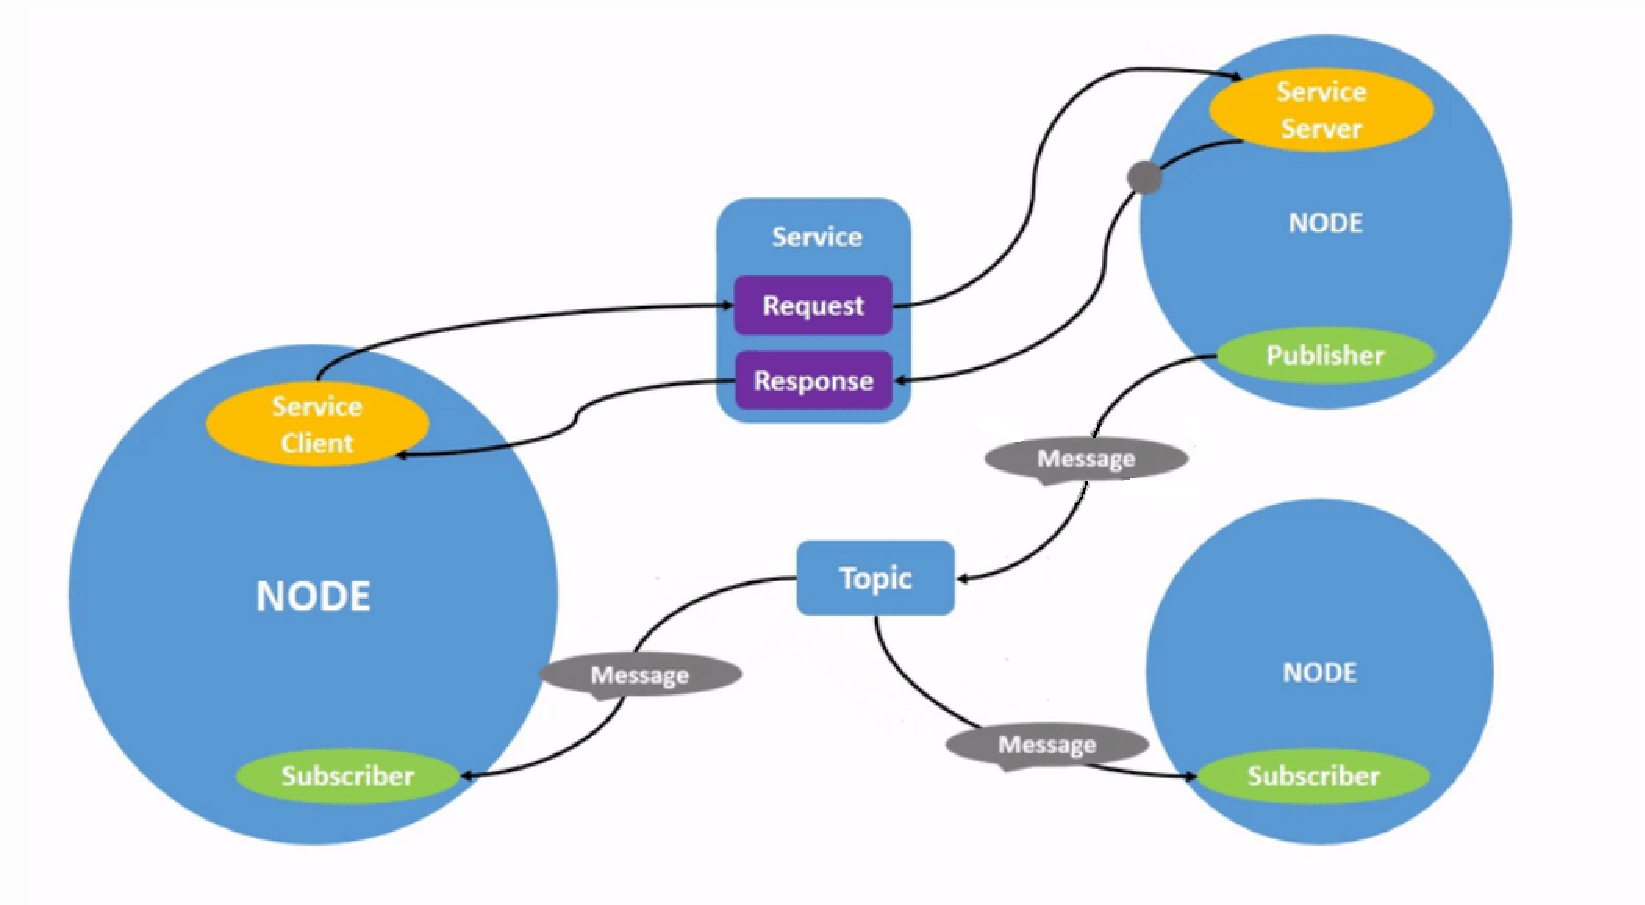
\includegraphics[width = 0.8\textwidth]{Figures/figROSConcept.pdf}
  \caption{Nodes, messages, topics and services. Nodes performs the computational tasks. Messages are sent to topics. Topics can be published and subscribed to by different nodes. Services contain a request and response message to preform synchronised communication between nodes. Figure from ROS 2 documentation, same principles apply for ROS \cite{ROS2Nodes}.}
  \label{fig:T:RC:Nodes}
\end{figure}

To increase security, and system up-time, ROS 2 was developed as a replacement to ROS \cite{MacenskiROS22022}. ROS 2 is based upon Data Distribution Service (DDS) for communication, which provides high security, embedded and real-time support as well as multi-robot communication. It builds on the familiar structure of nodes, messages, topics, services and tf2 transforms from ROS, but with additional functionality on top of this

Both ROS and ROS 2 contains large open source libraries of algorithms for common robotic applications like EKF, SLAM, manipulator planning and autonomous navigation to name a few. The algorithms are contained in structures called packages, which may contain several nodes, files for launching the nodes, parameters, and other content that may be needed to run the specific package.

ROS and ROS 2 provide development tools for visualisation, simulation, debugging, and more \cite{MacenskiROS22022} \cite{QuigleyROS}. Popular developer tools include Rviz for ROS and its ROS 2 port Rviz2. This is a graphical interface where developers can see 3D digital twins of their robot and visualise sensor data associated with he robot in real-time. Another popular tool for ROS and ROS 2 is Gazebo, a simulation environment where developers can simulate their robotic systems. RQT is another tool where the developer can visualise how nodes interact through topics and services in their robotic system.


\section{Autonomous Navigation} \label{sec:T:AutonomousNavigation}
% aj make it navigation, as you have a section - SLAM later that combines perception and this section
As pointed out in section \ref{sec:I:AutonomousNavigation}, for a mobile robot to be able to do autonomous navigation, there are four capabilities that needs to be set up. This section describes methods used to solve these problems in mobile robotics.

% In order to achieve autonomous navigation of a mobile robot, some requirements first has to be met. The robot needs to be able to estimate its own movement based on the kinematics of the vehicle and the encoder feedback from the wheels. This is done through the motion control system described in section \ref{sec:M:AN:MotionControl}. 
% The UGV needs some form of perception system to help determine its absolute position within the environment. This is done through the perception system described in section \ref{sec:M:AN:Perception}. Lastly,  to better estimate it's position in the environment and to give a map of the environment, some localisation and mapping systems should be implemented. This is described in section \ref{sec:M:AN:LocalisationAndMapping}. 

\subsection{Motion Control}\label{sec:T:AN:MotionControl}
Motion Control in mobile robotics refers to the actuation of motors to move around the environment in a controlled manner. The control system calculates the actuation of the robotic motors based on inverse kinematics, moves the mobile robot by actuating its motors and estimates its movement based on wheel measurements and forward kinematics.
The design of the mobile robot needs to be centred around the design requirement that the robot needs an efficient way of traversing it's intended environment in a predictable manner. Predictable is important as the robotic system needs to be able to estimate it's movement as accurately as possible. This section will introduce the reader to some common mechanisms of locomotion and a few mobile robotic designs.

\subsubsection{Locomotion}
The mechanisms that traverse the robot through the environment, is referred to as locomotion. Close to all mechanisms of locomotion are heavily inspired from nature. Examples of such locomotion mechanisms are walking, sliding, jumping, swimming and flying. Legged locomotion gives the benefit of adaptability and manoeuvrability in rough terrain. However, legged locomotion suffer from power inefficiency and high complexity. The human invention of powered wheel is simple and extremely energy efficient on hard surfaces and also not inspired by nature in contrast with many other locomotion mechanisms. Wheeled locomotion is therefore by far the most popular type of locomotion in mobile robotics\cite{SiegwartRoland2011Itam}. 

\subsubsection{Differential Drive Robots}\label{sec:T:AN:MRD:DifferentialDriveRobots}
Differential drive mobile robots refers to a wheeled robotic system made up of a rigid body with two driven wheels. Figure \ref{fig:differentialDrive} illustrates different types of differential drive robotic movement systems. The common denominator for all three of the robotic systems in figure \ref{fig:differentialDrive}, is that they all rely on two driven wheels.

\begin{figure}[htp]
  \centering
  \includesvg[width = 0.7\textwidth]{Figures/DifferentialDrive.drawio.svg}
  \caption{Illustration of different differential drive robotic designs. \textbf{a:} Two independently driven wheels in the rear/front, one unpowered omnidirectional wheel in the front/rear. \textbf{b:} Two-wheel centered differential drive with a third point of contact. \textbf{c:} Two-wheel differential drive with the center of mass (COM) below the axle. Figure inspired from \cite{SiegwartRoland2011Itam}.}
  \label{fig:differentialDrive}
\end{figure}

% Inspired by \cite{SiegwartRoland2011Itam}, the robot is modelled as a rigid body on wheels, interacting with a horizontal plane. The robot has a total of three DOFs, two for position, and one orientation along the orthogonal axis of the plane. Figure \ref{fig:PositionalRepresentation} illustrates how the robot is modelled and how the pose of the robot is specified on the plane. The axes $X_I$ and $Y_I$ represents a global reference frame on the plane with its origin at $O:{X_I, Y_X}$. A point P defined on the robot's chassis to act as a position reference point. Using the point P as origin, the axes $X_R$ and $Y:_R$ represents the robot's local reference frame. 

% \begin{figure}[htp]
%   \centering
%   \includesvg[width = 0.7\textwidth]{Figures/figPositionalRepresentation.drawio.svg}
%   \caption{Illustration of the local robot reference frame, $P:{X_R, Y_R}$, relative to the global reference frame, $O:{X_I, Y_I}$. The pose of the robot is given as $\zeta_I$ where $x$ and $y$ denotes position and $\theta$ denotes angular rotation of local frame relative to global frame. Figure inspired from \cite{SiegwartRoland2011Itam}.}
%   \label{fig:PositionalRepresentation}
% \end{figure}

% Looking at figure \ref{fig:PositionalRepresentation}, the position of $P$ is given as $P=(x,y)$ and the angle between the global and local reference frame is given as $\theta$. The pose of the robot becomes $\zeta_I$, where the subscript $I$ specifies that the pose is given relative to the global reference frame. Definition of $\zeta_I$ is given in eq. \ref{eq:posRep}.

% \begin{equation}
%     \label{eq:posRep}
%     \zeta_I &= \begin{bmatrix}
%                 x \\
%                 y \\
%                 \theta
%                 \end{bmatrix}
% \end{equation}


\subsubsection{Skidding Robots} \label{sec:T:AN:MRD:SkiddingRobots}
On a differential drive robot, the assumption is made that the driven wheels are not allowed to skid against the surface. However, there is an alternative type of robot where skidding is a part of the steering mechanism. Similarly to differential drive robots, these robots reorient themselves by spinning the wheels on each side of the robot at different speeds or in opposite directions. The difference is that these robots usually have tracks or several wheels on each side, giving it a much larger contact patch with the ground. The large contact patch gives these robots significantly improved traction in loose and rough terrain. Due to this large contact patch, the robot will usually skid when turning, hence the name. On some designs, the whole contact patch will be skidding when turning. This is the same type of locomotion that is used by military tanks\cite{SiegwartRoland2011Itam}. Figure \ref{fig:skidDrive} illustrates different skidding robot designs.

\begin{figure}[htp]
  \centering
  \includesvg[width = 0.7\textwidth]{Figures/skiddingDrive.drawio.svg}
  \caption{Illustration of different skidding robot designs. \textbf{a:} Tracked robot, \textbf{b:} Six wheeled robot, \textbf{c:} Four wheeled robot.}
  \label{fig:skidDrive}
\end{figure}
% aj change 1,2,3 to a,b,c
% ØØ - Done
The main disadvantage of these skidding robots is that their turning nature makes it difficult to determine a center of rotation. In addition, the turning motion will be affected by differences in surface friction. This makes it significantly harder to determine the exact pose of the robot when turning, compared to a normal differential drive robot. As a result, dead-reckoning is inaccurate for these robots and too aggressive turning motions could disorient the whole system. Another disadvantage is that the robot must overcome the static friction between the ground and the wheels/tracks to turn, this is highly inefficient on surfaces with high friction.


\subsection{Perception}\label{sec:T:AN:Perception}
In order to achieve autonomous navigation, it is essential for a robotic system to acquire knowledge of itself and its surroundings. Some examples of sensors used for mobile robot perception are Light Detection And Ranging (LiDAR) sensors and Ultrasonic sensors. An examples of use are; the popular mobile robot TurtleBot3 by the company ROBOTIS who utilise a 2D LiDAR for it's perception system\cite{turtlebot3RobotisManual}. \cite{Minghao2019LidarMob} who utilise a 3D LiDAR for the perception system in their mobile robot. \cite{Abueejela2018} who used an ultrasonic sensor to create a simple obstacle avoidance system for a simple wheeled robot.

Perception systems like the 3D LiDAR produces data sets on the form of a cloud of points called a point cloud. This is a collection of points in space that represents the range measurements from the sensor. For a 2D LiDAR, the data output is of the same type, but since this sensor measures a plane, its output is often called a laser scan.

% Laser Range Finders, often known as Light Detection And Ranging (LiDAR) sensors, are sensors that utilise light to measure the distance from the sensor to an obstacles. These sensors may use various principle, for example direct-time-of-flight. Direct time-of-flight LiDARs bases itself on directly measuring the round-trip time of a light pulse. The sensor transmits a light pulse and then measures the time it takes before this light pulse returns after bouncing off an obstacle. The distance, $d[m]$, between the sensor and the obstacle can then be calculated based on the speed of light $c=3X10^8[m/s]$, and the delta time, $\Delta t[s]$ as

% \begin{equation}\label{eq:TOF}
% d = \frac{c \cdot \Delta t}{2}.
% \end{equation}

% A two-dimensional LiDAR sensor can be made by rotating the sensor and mapping the measurements to the rotation. This can also be expanded to three dimensions by rotating a vertical array of sensors, creating a rotating vertical sensor beam. 



% Two different working principles are discussed in the following paragraphs; direct time-of-flight and indirect time-of-flight.

% The measurement is divided by two as the light travels the distance twice, to the obstacle and back. One disadvantage of this principle, at least for laser range finders, is that it places high requirements on the electronics of the sensors. As an example, if an obstacle is placed 1[m] away from the sensor, the round-trip time of the light pulse would be $\Delta t=6.667X10^{-9}[s]$. Accounting for the Nyquist–Shannon sampling theorem, which states that a measurement needs to be more than twice the frequency of the measured signal in order to be sufficient, since $f_{\Delta t}=150MHz$, the sampling frequency would have to be more than $B=300MHz$ in order to detect that signal. 

% Indirect time-of-flight sensors rely on emitting a modulated light wave and then looking at the phase shift of the returning measurement. The phase shift is directly related to the distance between the sensor and the object. Based on the phase shift $\phi[rad]$, the speed of light $c=3X10^8[m/s]$ and the modulation frequency $f_m[Hz]$, the distance between the sensor and the object can be calculated as

% \begin{equation}\label{eq:iTOF}
% d = \frac{c \cdot \phi}{2\pi \cdot 2 \cdot f_m}.
% \end{equation}
% In this case, the distance is also divided by two as the light travels twice the distance. Since the phase shift is measured in the frequency domain, several cycles of the modulated light pulse, are required to complete one measurement. This might prove impractical for some applications.



% aj add camera, radar, thermal camera


\subsection{Localisation and Mapping}\label{sec:T:AN:Localisation}
%aj i would suggest make the title simultaneous localization and mapping. Then odometry, ... kalman filter becomes the part of it
Robot localisation involves the robot building a map of the robot's environment, and determining its position relative to this map\cite{SiegwartRoland2011Itam}.  To achieve successful localisation, a combination of different localisation techniques is often used. As an example, a mobile robot could combine odometry estimates and LiDAR measurements to determine its position. The following paragraphs discuss some localisation implementations.

% \subsubsection{Wheel Encoders}
% To estimate chassis travel, an autonomous robot utilises rotational encoders to measure wheel movement. A rotational encoder may be based on one of many functional principles, but the common denominator for all rotational encoders are that they measure  rotational displacement. 
% % ØØ ---------- Might not need this?? --------

\subsection{Wheel Odometry}
Wheel odometry refers to the use of wheel sensors and forward kinematics to estimate the position of the robot over time. Wheel encoders are usually relative, meaning that they don't provide an absolute measurement on the displacement of the wheels. As a result, wheel odometry relies on integrating the wheel movement over time and then using this together with forward kinematics to calculate the robots pose. The accuracy of this pose estimation method is highly dependant on the mobile robot's design and the wheel sensor accuracy. Because of the integration, the measurement errors accumulate over time, making wheel odometry drift over time. % Do i need sources??

\subsubsection{Inertial Measurement Unit}
An Inertial Measurement Unit (IMU) is a device that combines accelerometers, gyroscopes and magnetometers to measure the acceleration, angular movement and orientation of a body. IMUs are often used to help determine the localisation of vehicles, and robots. Using IMU measurements, the movement of an object can be estimated by integration over time, as with wheel odometry. Similarly to wheel odometry, the measurement errors is integrated over time resulting in drift.
% Do i need sources for this or is it fine?


\subsubsection{Kalman Filter \& Extended Kalman Filter}
An Extended Kalman Filter (EKF) is often used in robotics to fuse several sensor measurements and estimations to one optimal estimate. This way, no one measurement has to be chosen and no measurements has to be discarded. To understand what an EKF is, one must first have an understanding about traditional Kalman Filters. A Kalman Filter utilises a Gaussian distribution to represent the belief of the robots location. A Gaussian only has two parameters, its mean $\mu$, a covariance $\Sigma$. As there are only two parameters that are updated during each prediction, this results in a very efficient algorithm. However, it also means that the filter needs to have an initial belief that is close to it's actual position in order to be effective. It also has no way of recovering it's position if it gets lost. Appendix \ref{A:KalmanFilterLocalisation} contains a figure illustrating one-dimensional Kalman Filter Localisation, including some explanation around this.
Kalman Filters assume the system to be linear and with white Gaussian noise. However, most robotic applications are nonlinear. The algorithm therefore has to linearise the system before applying the Kalman Filter \cite{SiegwartRoland2011Itam}. This extension to the original Kalman Filter gives it the name EKF. Linearisation is a simplification of what could otherwise be a complex n-th order system. The result is that the EKF may only work within a certain operating range of the system and may not be helpful at all for some systems. %For more info on Kalman Filters and EKFs, see \cite{SiegwartRoland2011Itam} or \cite{ThrunSebastian2005Pr}.
Examples of use of EKF in localisation are \cite{ApolloEKF1973} who used a version of EKF on the Apollo 10 and 11 missions. For mobile robots, EKF is successfully used to counter wheel odometry and IMU drift \cite{Chen2012}.

\subsubsection{Monte Carlo Localisation}
EKFs are computationally efficient and a great tool to improve probabilistic localisation. However, an EKF based localisation would not be able to do \textit{global localisation} (initial position is unknown, \cite{SiegwartRoland2011Itam}, \cite{ThrunSebastian2005Pr}) or solve the \textit{kidnapped robot problem} (robot gets kidnapped and moved to another location \cite{SiegwartRoland2011Itam} \cite{ThrunSebastian2005Pr}). In this case, a particle-based localisation method like Monte Carlo Localisation (MCL) has proven to be successful. The method bases itself on randomly distributing a set of particles in the free configuration space. It then gives each particle a weight based on the possibility that the robot is located at the respective particle. Next, it re-samples the particles, but with more particles around the areas where particles had the strongest weighting from the previous belief. This is done until a major part of the cumulative particle mass is centred around one location belief. Appendix \ref{A:MonteCarloLocalisation} contains a figure illustrating one-dimensional MCL including some explanation.

Plain MCL use particle sample sets of fixed size. At an early stage of localisation, when the robot does not know where it is, the sample set needs to be large to avoid divergence. However, when the location of the robot is fairly confident or known, it is computationally inefficient to have an unnecessarily large particle set. A variant of MCL, called KLD-sampling MCL, adapts the number of particles based on Kullback-Leibler divergence (KLD). Kullback-Leibler divergence is a measure of the difference between two probability distributions. KLD-sampling use KLD to create a measure for the difference between the true posterior belief provided by measurements, and the sample-based approximation of this belief. To read more about this localisation method, please refer to \cite{ThrunSebastian2005Pr}. Examples of use of KLD-Sampling MCL for mobile robot localisation are \cite{Wasisto2019}, \cite{NAV2020}, \cite{Song2017}.

\subsubsection{Simultaneous Localisation and Mapping} \label{sec:T:AN:L:SLAM}
Both EKF-localisation and MCL assumes that it is given a map of the environment. Although there could be a pre-made map that fits the application, this is often not the case. The robot therefore has to do the mapping and localisation at the same time. This problem is called the Simultaneous Localisation and Mapping problem (SLAM problem). One of the more popular solutions to the SLAM problem is by the use of pose graphs \cite{Konolige2010}. A pose graph is a sparse graph of nodes with constraints between them. The nodes in the graph are different robot poses and features of the map. The constraints represent the relative relation between the robot poses and also between robot poses and features of the map. It is important to specify that the constraints between the poses are non-rigid. The pose graph can therefore be interpreted as an elastic net of poses. The solution is then to find the state where this net has the minimum amount of energy \cite{SiegwartRoland2011Itam}. Figure \ref{fig:poseGraph} illustrates how a pose graph is built from different robot poses and map-feature poses as a robot moves through an environment. As the map becomes larger, the size of the pose graph also increases, which in turn results in an increased computational effort required for optimisation. A method of pose graph optimisation that has proven to be efficient, is Sparse Pose Adjustment (SPA)\cite{Konolige2010}. A map can be constructed as for example an occupancy grid map (described in \cite{ThrunSebastian2005Pr}), after the pose graph has been constructed and optimised. 

\begin{figure}[htp]
  \centering
  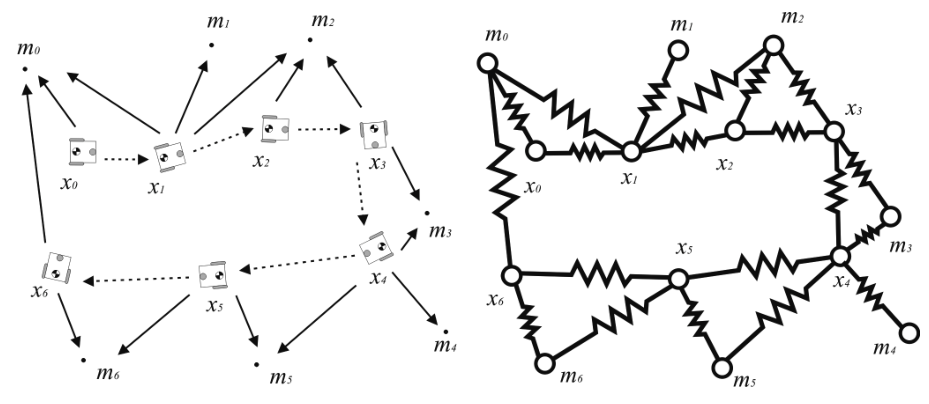
\includegraphics[width = 0.9\textwidth]{Figures/figposeGraph.pdf}
  \caption{Demonstration of pose graph. The illustration demonstrates how robot and map feature poses are presented as nodes with flexible constraints between them to generate a pose graph. Robot poses are denoted as $x_i$ and map feature poses are denoted as $m_n$. Figure from \cite{SiegwartRoland2011Itam}.}
  \label{fig:poseGraph}
\end{figure}

% \subsection{Obstacle Avoidance} \label{sec:T:AN:PP:ObstacleAvoidance}
% Obstacle avoidance refers to the act of avoiding obstacles that are detected by the robot's sensors in order to avoid collision. As an example, if a pedestrian is standing in the robot's trajectory, then the local planner divert the robot so that it moves around the pedestrian instead of running into it. After the evasive action has taken place, the robot should have adjusted it's trajectory so that it can keep following it to reach it's goal. A popular method for obstacle avoidance is the dynamic window approach. This approach takes 

% \section{Pick and Place}
% In the context of this thesis, pick and place refers to the complete pipeline of searching for and detecting an object using computer vision, picking it using a robotic manipulator, and placing the object on another location. This section will introduce some different methods for object detection and mention some core concepts on robotic manipulation that is necessary to understand when delving into the work of this thesis.

\section{Computer Vision} \label{sec:T:MachineVision}
Computer vision refers to giving machines the ability to process an image and reporting back what it sees \cite{SnyderWesleyE.2010Mv}. The objective of computer vision systems may vary based on the application. For example, the objective might be to locate an object, classifying different objects, inspect objects, and much more. In recent years, point cloud data have also been used to preform computer vision tasks, often in combination with machine learning.

\subsubsection{Machine Learning Based Object Detection \& Pose Estimation} \label{sec:T:MV:CNN-based}
Machine learning based approaches for object detection and 6-DOF pose estimation has been researched extensively in recent years and have the possibility to provide robust detection solutions. Some solutions could be used with normal monocular cameras, for example \cite{JosipKerzel2018}, who combines a 2D CNN detector and before a CNN model trained for viewpoint estimation is used to achieve pose estimation in monocular images. Other solutions combine image data with 3D point clouds, such as \cite{WeiDuan2020}. Similarly to \cite{JosipKerzel2018}, this solution first detects the object using a 2D CNN detector for images, then their network will determine the object's pose and deliver a segmented point cloud highlighting the object.

\subsubsection{Fiducial Tag Based Object Detection }\label{sec:T:OD:TagBasedObjectDetection}
Fiducials are artificial features designed to be easy to detect by a computer vision systems \cite{krogius2019iros}. Among the more popular fiducial tag systems are ArUco, \cite{JuardoSalinas2016} \cite{RamirezSalinas2018},  and AprilTags \cite{olson2011tags} \cite{wang2016iros} \cite{krogius2019iros}. These fiducial tags come in different shapes, in the case of AprilTags, some different tag types are shown in figure \ref{fig:T:PAP:MV:AprilTag}. The differnt tag types from figure \ref{fig:T:PAP:MV:AprilTag} are defined as tag families. Each of these tag families have a large collection of pre-defined tags for developers to use for their respective projects.

\begin{figure}[htp]
  \centering
  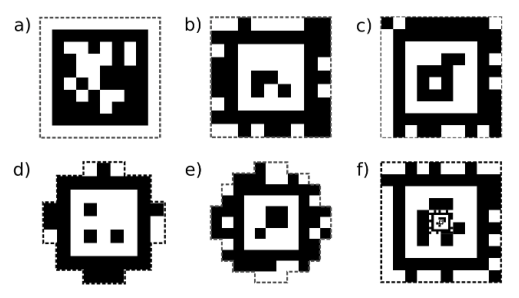
\includegraphics[width = 0.7\textwidth]{Figures/figAprilTag.pdf}
  \caption{Different AprilTag types. The types are defined in different tag families. Their respective families are defined as: \textbf{a)} Tag36h11, common square tag. \textbf{b)} TagStandard41h12 and \textbf{c)} TagStandard52h12, square tags with one layer of bits around border. \textbf{d)} TagCircle21h7 and \textbf{e)} TagCircle49h12, circular tags. \textbf{f)} TagCustom48h12, tag with possibility of smaller tag in the middle. Figure along with adapted explanation from \cite{krogius2019iros}.}
  \label{fig:T:PAP:MV:AprilTag}
\end{figure}



% \section{Rapidly Exploring Random Tree}
% Rapidly Exloring Random Tree involvels growing a single tree from start to find a motion to the goal in $C_{free}$. It uses a sampler to sample randon point in the free space, then an algorithm find the node in the tree closes to the random point. The planner then adds a new node towards the random point at a defined distance from the existing node. A local planning algorithm is then used to connect the existing node to the new node. This operation is done until a feasible path is found. Variations of this method exists, such as bidirectional RRT, which expands two trees, one from start and one from goal. As well as RRT*, which will optimise the path as it finds shorter paths to the branches of the tree. RRT* will converge towards an optimal solution as time goes to infinity \cite{LynchKevin2017Mr:m}.



% \section{Robot Operating System 2}
% Robot operating system 2 is an open source operating system for robots that is aimed at simplifying the communication between different sensors and actuators in a robotic system, and present the information from these different sensors and actuators in a standardised matter.
% % aj not needed

% \subsection{URDF}
% % aj not needed


%\section{Conclusion}
% we described the building block that forms the basis of our Thesis aimed towards warehouse automation - perception, autonomous navigation, object localization, robotic manipulation. each chapter should have an introduction mentioning what IS covered and end with conclusion mentioning what WAS covered.